\vsssub
\subsubsection{~Shoreline reflection} \label{sub:num_refl}
\conthead{???}{F. Ardhuin}

\noindent
In the case of icebergs and sub-grid islands, the reflected energy is
redistributed evenly in all directions within 90$\degree$ of the direction
opposite to the incoming waves.  For resolved lands, a mean direction
perpendicular to shore $\theta_n$ was defined from the land or sea status of
the 8 grid points surrounding the local point (Fig. \ref{fig:refl}).

For each model grid point adjacent to land, the analysis of the land-sea
geometry gives one value of $\theta_n$ among 16 possible directions. Together
with any incoming wave direction $\theta_i$ this defines a specular reflection
direction $\theta_r=2 \theta_n - \theta_i + \pi$.  For each spectral component
of direction $\theta_i$ going towards the coast (i.e. such that
$\cos(\theta_i-\theta_n) >0$), the total reflection is $R^2$ times the
incoming energy. This reflected energy $R^2 E(f) M(f,\theta_i)$ is
redistributed over directions around the specular reflection direction
$\theta_r$, with a broad distribution taken proportional to
$\cos^n(\theta-\theta_r)$, where the power $n$ is a function of the local
shoreline geometry.

\begin{figure} \begin{center}
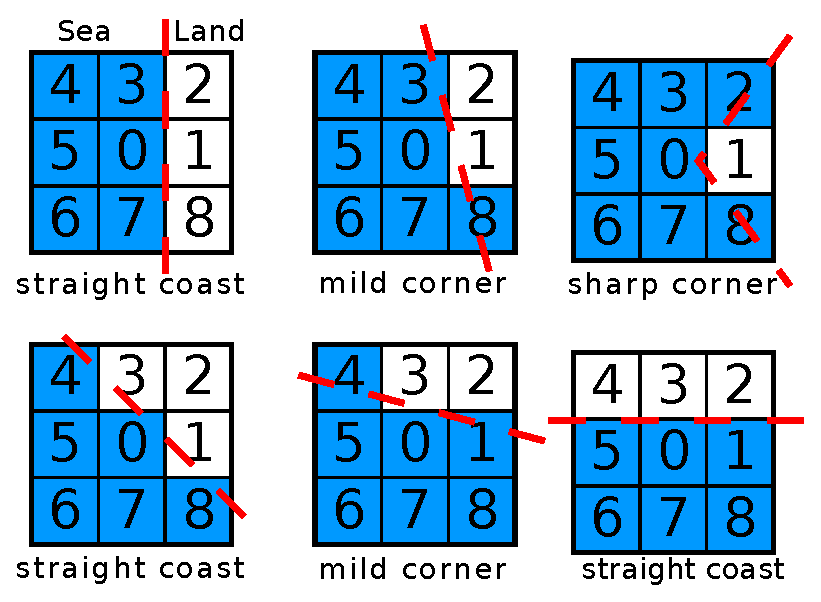
\epsfig{file=./num/coast_reflection.eps,angle=0,width=3in}
\caption{Examples of determination of the shoreline orientation and geometry
  using the land / sea mask. For any sea point (number 0) which is the ocean
  (in blue) and has at least one neighbor in land (in white) the eight
  neighbors, numbered from 1 to 8 are used to define the shoreline geometry.
  For `mild' corners and straight coasts, the estimated shoreline orientation
  (dashed line) is used to compute the directional distribution of the
  reflected wave energy.  }
\label{fig:refl} \botline
\end{center}
\end{figure}

For this purpose we distinguish three different shoreline geometries relative
to the local point as illustrated by figure \ref{fig:refl}: we set $n=2$ for a
straight coast (three connected land points among the neighbors), $n=1$ for a
mild corner (two land points among the neighbors), and $n=0$ at a sharp corner
(only one land point, among the 4 closest neighbors) which corresponds to the
same treatment done for sub-grid islands and icebergs. Changing these values
of $n$ in the range $0$ to $2$ has little effects on our results.  $n=1$
corresponds to a Lambertian surface approximation, which is used for
electromagnetic wave scattering from rough surfaces. A pure specular
reflection would be obtained with $n$ infinite.  A more rigorous treatment
should use the distribution of the shoreline orientation at at the scale of
the ocean wavelength, namely of the order of 100~m.